% Options for packages loaded elsewhere
\PassOptionsToPackage{unicode}{hyperref}
\PassOptionsToPackage{hyphens}{url}
%
\documentclass[
  man,floatsintext]{apa6}
\usepackage{amsmath,amssymb}
\usepackage{lmodern}
\usepackage{iftex}
\ifPDFTeX
  \usepackage[T1]{fontenc}
  \usepackage[utf8]{inputenc}
  \usepackage{textcomp} % provide euro and other symbols
\else % if luatex or xetex
  \usepackage{unicode-math}
  \defaultfontfeatures{Scale=MatchLowercase}
  \defaultfontfeatures[\rmfamily]{Ligatures=TeX,Scale=1}
\fi
% Use upquote if available, for straight quotes in verbatim environments
\IfFileExists{upquote.sty}{\usepackage{upquote}}{}
\IfFileExists{microtype.sty}{% use microtype if available
  \usepackage[]{microtype}
  \UseMicrotypeSet[protrusion]{basicmath} % disable protrusion for tt fonts
}{}
\makeatletter
\@ifundefined{KOMAClassName}{% if non-KOMA class
  \IfFileExists{parskip.sty}{%
    \usepackage{parskip}
  }{% else
    \setlength{\parindent}{0pt}
    \setlength{\parskip}{6pt plus 2pt minus 1pt}}
}{% if KOMA class
  \KOMAoptions{parskip=half}}
\makeatother
\usepackage{xcolor}
\usepackage{longtable,booktabs,array}
\usepackage{calc} % for calculating minipage widths
% Correct order of tables after \paragraph or \subparagraph
\usepackage{etoolbox}
\makeatletter
\patchcmd\longtable{\par}{\if@noskipsec\mbox{}\fi\par}{}{}
\makeatother
% Allow footnotes in longtable head/foot
\IfFileExists{footnotehyper.sty}{\usepackage{footnotehyper}}{\usepackage{footnote}}
\makesavenoteenv{longtable}
\usepackage{graphicx}
\makeatletter
\def\maxwidth{\ifdim\Gin@nat@width>\linewidth\linewidth\else\Gin@nat@width\fi}
\def\maxheight{\ifdim\Gin@nat@height>\textheight\textheight\else\Gin@nat@height\fi}
\makeatother
% Scale images if necessary, so that they will not overflow the page
% margins by default, and it is still possible to overwrite the defaults
% using explicit options in \includegraphics[width, height, ...]{}
\setkeys{Gin}{width=\maxwidth,height=\maxheight,keepaspectratio}
% Set default figure placement to htbp
\makeatletter
\def\fps@figure{htbp}
\makeatother
\setlength{\emergencystretch}{3em} % prevent overfull lines
\providecommand{\tightlist}{%
  \setlength{\itemsep}{0pt}\setlength{\parskip}{0pt}}
\setcounter{secnumdepth}{-\maxdimen} % remove section numbering
% Make \paragraph and \subparagraph free-standing
\ifx\paragraph\undefined\else
  \let\oldparagraph\paragraph
  \renewcommand{\paragraph}[1]{\oldparagraph{#1}\mbox{}}
\fi
\ifx\subparagraph\undefined\else
  \let\oldsubparagraph\subparagraph
  \renewcommand{\subparagraph}[1]{\oldsubparagraph{#1}\mbox{}}
\fi
\newlength{\cslhangindent}
\setlength{\cslhangindent}{1.5em}
\newlength{\csllabelwidth}
\setlength{\csllabelwidth}{3em}
\newlength{\cslentryspacingunit} % times entry-spacing
\setlength{\cslentryspacingunit}{\parskip}
\newenvironment{CSLReferences}[2] % #1 hanging-ident, #2 entry spacing
 {% don't indent paragraphs
  \setlength{\parindent}{0pt}
  % turn on hanging indent if param 1 is 1
  \ifodd #1
  \let\oldpar\par
  \def\par{\hangindent=\cslhangindent\oldpar}
  \fi
  % set entry spacing
  \setlength{\parskip}{#2\cslentryspacingunit}
 }%
 {}
\usepackage{calc}
\newcommand{\CSLBlock}[1]{#1\hfill\break}
\newcommand{\CSLLeftMargin}[1]{\parbox[t]{\csllabelwidth}{#1}}
\newcommand{\CSLRightInline}[1]{\parbox[t]{\linewidth - \csllabelwidth}{#1}\break}
\newcommand{\CSLIndent}[1]{\hspace{\cslhangindent}#1}
\ifLuaTeX
\usepackage[bidi=basic]{babel}
\else
\usepackage[bidi=default]{babel}
\fi
\babelprovide[main,import]{english}
% get rid of language-specific shorthands (see #6817):
\let\LanguageShortHands\languageshorthands
\def\languageshorthands#1{}
% Manuscript styling
\usepackage{upgreek}
\captionsetup{font=singlespacing,justification=justified}

% Table formatting
\usepackage{longtable}
\usepackage{lscape}
% \usepackage[counterclockwise]{rotating}   % Landscape page setup for large tables
\usepackage{multirow}		% Table styling
\usepackage{tabularx}		% Control Column width
\usepackage[flushleft]{threeparttable}	% Allows for three part tables with a specified notes section
\usepackage{threeparttablex}            % Lets threeparttable work with longtable

% Create new environments so endfloat can handle them
% \newenvironment{ltable}
%   {\begin{landscape}\centering\begin{threeparttable}}
%   {\end{threeparttable}\end{landscape}}
\newenvironment{lltable}{\begin{landscape}\centering\begin{ThreePartTable}}{\end{ThreePartTable}\end{landscape}}

% Enables adjusting longtable caption width to table width
% Solution found at http://golatex.de/longtable-mit-caption-so-breit-wie-die-tabelle-t15767.html
\makeatletter
\newcommand\LastLTentrywidth{1em}
\newlength\longtablewidth
\setlength{\longtablewidth}{1in}
\newcommand{\getlongtablewidth}{\begingroup \ifcsname LT@\roman{LT@tables}\endcsname \global\longtablewidth=0pt \renewcommand{\LT@entry}[2]{\global\advance\longtablewidth by ##2\relax\gdef\LastLTentrywidth{##2}}\@nameuse{LT@\roman{LT@tables}} \fi \endgroup}

% \setlength{\parindent}{0.5in}
% \setlength{\parskip}{0pt plus 0pt minus 0pt}

% Overwrite redefinition of paragraph and subparagraph by the default LaTeX template
% See https://github.com/crsh/papaja/issues/292
\makeatletter
\renewcommand{\paragraph}{\@startsection{paragraph}{4}{\parindent}%
  {0\baselineskip \@plus 0.2ex \@minus 0.2ex}%
  {-1em}%
  {\normalfont\normalsize\bfseries\itshape\typesectitle}}

\renewcommand{\subparagraph}[1]{\@startsection{subparagraph}{5}{1em}%
  {0\baselineskip \@plus 0.2ex \@minus 0.2ex}%
  {-\z@\relax}%
  {\normalfont\normalsize\itshape\hspace{\parindent}{#1}\textit{\addperi}}{\relax}}
\makeatother

% \usepackage{etoolbox}
\makeatletter
\patchcmd{\HyOrg@maketitle}
  {\section{\normalfont\normalsize\abstractname}}
  {\section*{\normalfont\normalsize\abstractname}}
  {}{\typeout{Failed to patch abstract.}}
\patchcmd{\HyOrg@maketitle}
  {\section{\protect\normalfont{\@title}}}
  {\section*{\protect\normalfont{\@title}}}
  {}{\typeout{Failed to patch title.}}
\makeatother

\usepackage{xpatch}
\makeatletter
\xapptocmd\appendix
  {\xapptocmd\section
    {\addcontentsline{toc}{section}{\appendixname\ifoneappendix\else~\theappendix\fi\\: #1}}
    {}{\InnerPatchFailed}%
  }
{}{\PatchFailed}
\keywords{Diabetes, access to care, inflammation, health, Mexico, China\newline\indent Word count: X (this cannot easily be done automatically, we can also just leave it out)}
\usepackage{csquotes}
\usepackage[titles]{tocloft}
\cftpagenumbersoff{figure}
\renewcommand{\cftfigpresnum}{\itshape\figurename\enspace}
\renewcommand{\cftfigaftersnum}{.\space}
\setlength{\cftfigindent}{0pt}
\setlength{\cftafterloftitleskip}{0pt}
\settowidth{\cftfignumwidth}{Figure 10.\qquad}
\cftpagenumbersoff{table}
\renewcommand{\cfttabpresnum}{\itshape\tablename\enspace}
\renewcommand{\cfttabaftersnum}{.\space}
\setlength{\cfttabindent}{0pt}
\setlength{\cftafterloftitleskip}{0pt}
\settowidth{\cfttabnumwidth}{Table 10.\qquad}
\ifLuaTeX
  \usepackage{selnolig}  % disable illegal ligatures
\fi
\IfFileExists{bookmark.sty}{\usepackage{bookmark}}{\usepackage{hyperref}}
\IfFileExists{xurl.sty}{\usepackage{xurl}}{} % add URL line breaks if available
\urlstyle{same} % disable monospaced font for URLs
\hypersetup{
  pdftitle={Relations between Inflammation, access to care and Diabetes in two repesentative populations of China and Mexico.},
  pdfauthor={Dominik Grätz1, Rachel Miller-Moudgil1, Amber Somarriba1, Brittany Spinner1, \& Tian Walker1},
  pdflang={en-EN},
  pdfkeywords={Diabetes, access to care, inflammation, health, Mexico, China},
  hidelinks,
  pdfcreator={LaTeX via pandoc}}

\title{Relations between Inflammation, access to care and Diabetes in two repesentative populations of China and Mexico.}
\author{Dominik Grätz\textsuperscript{1}, Rachel Miller-Moudgil\textsuperscript{1}, Amber Somarriba\textsuperscript{1}, Brittany Spinner\textsuperscript{1}, \& Tian Walker\textsuperscript{1}}
\date{}


\shorttitle{Inflammation, access to care and Diabetes in China and Mexico.}

\authornote{List of group members ordered by alphabet.}

\affiliation{\vspace{0.5cm}\textsuperscript{1} University of Oregon}

\abstract{%
\emph{Background.} Background goes here. \emph{Methods.} Methods go here. \emph{Results.} Results here. \emph{Conclusions.} Conclusions here.
}



\begin{document}
\maketitle

\hypertarget{introduction}{%
\section{Introduction}\label{introduction}}

Enter text/code here. I make a reference here (Deshpande, Harris-Hayes, \& Schootman, 2008).
\textbf{This is just copied from the outline document; needs to be rewritten/references automated!}

\hypertarget{about-the-data}{%
\subsection{About the data:}\label{about-the-data}}

We will be using two datasets from the Wave 1 Study on Global Ageing (SAGE) from the World Health Organization (WHO). We will be looking at inflammation (measured through C-reactive protein; crp) and hemoglobin A1c (average blood glucose level over the last three months) to better understand the relationship between inflammation and diabetes in Mexico and China. Observations of the potential association between diabetes and inflammation were initially made over 100 years ago (Williamson, 1901), and we now know that inflammation is a pathogenic mediator in the progression of diabetes, and likely has a causal role in some cases as well (Tsalamandris et al., 2019). The relationship between inflammation and diabetes is multifaceted but we know that decreasing inflammation means decreasing diabetes progression and complications (Agrawal \& Kant, 2014).
The data is from two datasets designed exactly the same: one from Mexico and one from China. The data frame for China has 13,367 observations from 1,489 variables. In the dataset from Mexico there are 2,315 observations of 1690 variables. Everything else is the same as the dataset from China. Almost all of the variables are numbers or characters, and the data was originally formatted in SPSS (statistical package for the social sciences). There were more people who did the survey than did the biomarker collection (source of CRP and HbA1c data) so the number of data points in our study is smaller than the full dataset. There is demographic information along with many health-related validated scales. We have listed the variables that we will be looking at below

\hypertarget{why-china-and-mexico}{%
\subsection{Why China and Mexico?}\label{why-china-and-mexico}}

China and Mexico are interesting places to study the relationship between diabetes and inflammation because they are both classified as low to middle income countries (LMIC's) where 80\% of the global burden of diabetes falls. Additionally, diabetes is a leading cause of death in Mexico and closely linked to the obesity epidemic. China experienced a famine that likely created an epigenetic environment that makes people prone to diabetes. Obesity is a relatively new phenomenon in China and so the pathophysiology of disease development may be different than other places where obesity has been a major issue for decades.

\hypertarget{methods}{%
\section{Methods}\label{methods}}

\hypertarget{results}{%
\section{Results}\label{results}}

Enter text/code here. Let's do all the coding here!

\begin{verbatim}
## 
## Call:
## lm(formula = crp ~ hba1c + medication, data = data_dia[data_dia$country == 
##     "China", ])
## 
## Residuals:
##     Min      1Q  Median      3Q     Max 
## -1.7485 -0.9752 -0.3596  0.7661  3.2601 
## 
## Coefficients:
##             Estimate Std. Error t value Pr(>|t|)    
## (Intercept)  1.38413    0.20967   6.602 1.34e-10 ***
## hba1c        0.03325    0.03060   1.087   0.2778    
## medication2 -0.30649    0.16159  -1.897   0.0586 .  
## ---
## Signif. codes:  0 '***' 0.001 '**' 0.01 '*' 0.05 '.' 0.1 ' ' 1
## 
## Residual standard error: 1.189 on 388 degrees of freedom
##   (103 observations deleted due to missingness)
## Multiple R-squared:  0.01352,    Adjusted R-squared:  0.008432 
## F-statistic: 2.658 on 2 and 388 DF,  p-value: 0.07136
\end{verbatim}

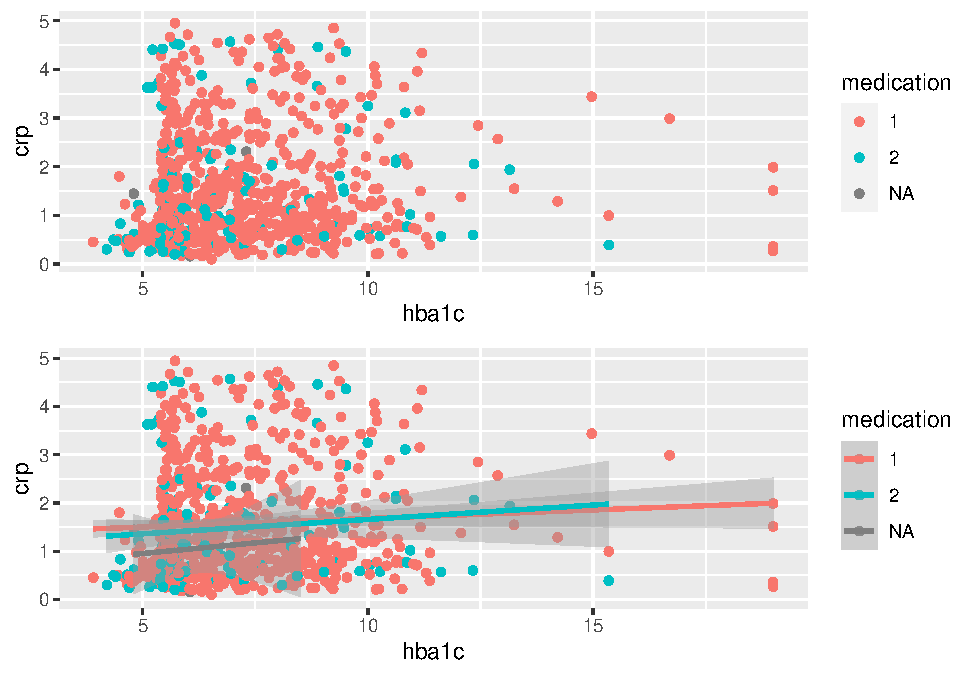
\includegraphics{Final_Groupof5_files/figure-latex/Reg1_HBA1C-CRP-1.pdf}

\begin{table}[tbp]

\begin{center}
\begin{threeparttable}

\caption{\label{tab:Table for Mreg1}This is where the caption goes}

\begin{tabular}{lllllll}
\toprule
Predictor & \multicolumn{1}{c}{$b$} & \multicolumn{1}{c}{95\% CI} & \multicolumn{1}{c}{$t$} & \multicolumn{1}{c}{$\mathit{df}$} & \multicolumn{1}{c}{$p$} & \multicolumn{1}{c}{predictor}\\
\midrule
Intercept & 1.38 & {}[0.97, 1.80] & 6.60 & 388 & < .001 & Intercept\\
Hba1c & 0.03 & {}[-0.03, 0.09] & 1.09 & 388 & .278 & Hba1c\\
Medication2 & -0.31 & {}[-0.62, 0.01] & -1.90 & 388 & .059 & Medication\\
\bottomrule
\addlinespace
\end{tabular}

\begin{tablenotes}[para]
\normalsize{\textit{Note.} Model fit: $F$(2, 388) = 2.66, $p$ = 0.07, $R^2$ = 0.01}
\end{tablenotes}

\end{threeparttable}
\end{center}

\end{table}

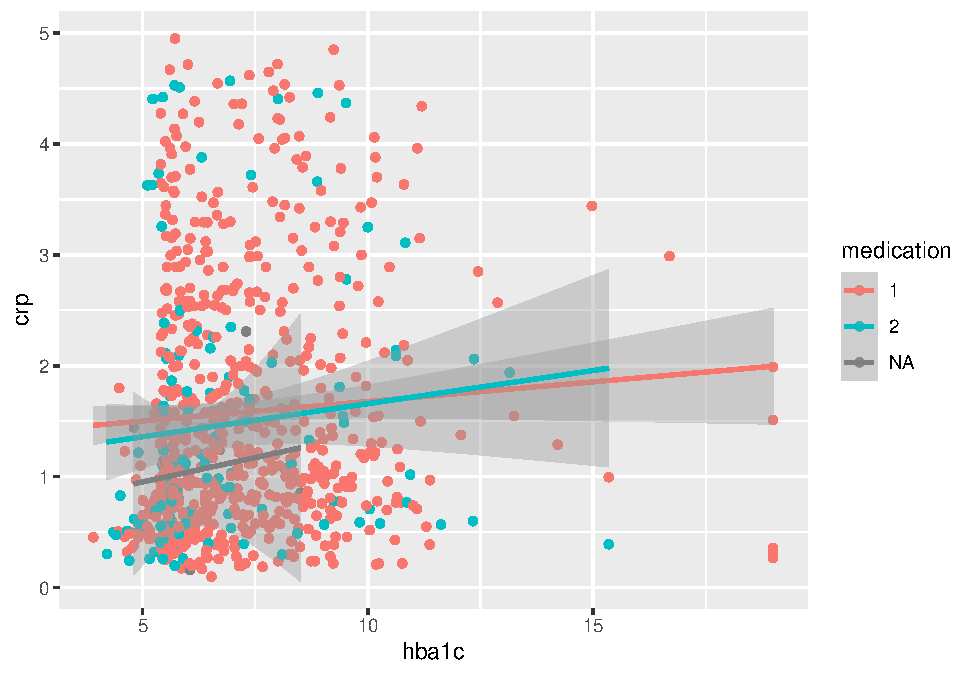
\includegraphics{Final_Groupof5_files/figure-latex/unnamed-chunk-5-1.pdf}

\begin{verbatim}
## 
## Call:
## lm(formula = crp ~ hba1c, data = mexico)
## 
## Residuals:
##     Min      1Q  Median      3Q     Max 
## -2.2072 -1.1830 -0.6649  0.5873  7.9933 
## 
## Coefficients:
##             Estimate Std. Error t value Pr(>|t|)    
## (Intercept)  1.38948    0.16425   8.459  < 2e-16 ***
## hba1c        0.09642    0.02564   3.761 0.000173 ***
## ---
## Signif. codes:  0 '***' 0.001 '**' 0.01 '*' 0.05 '.' 0.1 ' ' 1
## 
## Residual standard error: 1.808 on 2402 degrees of freedom
##   (3044 observations deleted due to missingness)
## Multiple R-squared:  0.005854,   Adjusted R-squared:  0.00544 
## F-statistic: 14.14 on 1 and 2402 DF,  p-value: 0.0001735
\end{verbatim}

\begin{verbatim}
## 
## Call:
## lm(formula = crp ~ hba1c, data = china)
## 
## Residuals:
##     Min      1Q  Median      3Q     Max 
## -3.0866 -1.2185 -0.8918  0.3402  8.4252 
## 
## Coefficients:
##             Estimate Std. Error t value Pr(>|t|)    
## (Intercept)  1.13766    0.08207  13.862  < 2e-16 ***
## hba1c        0.10663    0.01379   7.733 1.18e-14 ***
## ---
## Signif. codes:  0 '***' 0.001 '**' 0.01 '*' 0.05 '.' 0.1 ' ' 1
## 
## Residual standard error: 2.117 on 7547 degrees of freedom
##   (7501 observations deleted due to missingness)
## Multiple R-squared:  0.007862,   Adjusted R-squared:  0.00773 
## F-statistic:  59.8 on 1 and 7547 DF,  p-value: 1.185e-14
\end{verbatim}

\begin{verbatim}
## 
## Call:
## lm(formula = crp ~ hba1c + q_mean, data = data)
## 
## Residuals:
##     Min      1Q  Median      3Q     Max 
## -2.0621 -0.7793 -0.4305  0.4763  3.7343 
## 
## Coefficients:
##             Estimate Std. Error t value Pr(>|t|)    
## (Intercept) 0.698830   0.055714  12.543  < 2e-16 ***
## hba1c       0.064692   0.007052   9.174  < 2e-16 ***
## q_mean      0.164575   0.025041   6.572 5.27e-11 ***
## ---
## Signif. codes:  0 '***' 0.001 '**' 0.01 '*' 0.05 '.' 0.1 ' ' 1
## 
## Residual standard error: 1.099 on 7893 degrees of freedom
##   (1128 observations deleted due to missingness)
## Multiple R-squared:  0.01633,    Adjusted R-squared:  0.01608 
## F-statistic:  65.5 on 2 and 7893 DF,  p-value: < 2.2e-16
\end{verbatim}

\begin{verbatim}
## 
## Call:
## lm(formula = crp ~ hba1c + q_mean, data = mexico)
## 
## Residuals:
##     Min      1Q  Median      3Q     Max 
## -1.6072 -0.8459 -0.3834  0.5013  3.4315 
## 
## Coefficients:
##             Estimate Std. Error t value Pr(>|t|)    
## (Intercept)  1.16974    0.14278   8.193 4.78e-16 ***
## hba1c        0.04153    0.01903   2.182   0.0292 *  
## q_mean       0.10085    0.04422   2.281   0.0227 *  
## ---
## Signif. codes:  0 '***' 0.001 '**' 0.01 '*' 0.05 '.' 0.1 ' ' 1
## 
## Residual standard error: 1.173 on 1803 degrees of freedom
##   (22 observations deleted due to missingness)
## Multiple R-squared:  0.00579,    Adjusted R-squared:  0.004687 
## F-statistic:  5.25 on 2 and 1803 DF,  p-value: 0.00533
\end{verbatim}

\begin{verbatim}
## 
## Call:
## lm(formula = crp ~ hba1c + q_mean, data = china)
## 
## Residuals:
##     Min      1Q  Median      3Q     Max 
## -1.8911 -0.7416 -0.4657  0.4685  3.7628 
## 
## Coefficients:
##             Estimate Std. Error t value Pr(>|t|)    
## (Intercept)  0.82424    0.06612  12.466  < 2e-16 ***
## hba1c        0.05585    0.00757   7.378 1.82e-13 ***
## q_mean       0.06444    0.03349   1.924   0.0544 .  
## ---
## Signif. codes:  0 '***' 0.001 '**' 0.01 '*' 0.05 '.' 0.1 ' ' 1
## 
## Residual standard error: 1.067 on 6087 degrees of freedom
##   (1106 observations deleted due to missingness)
## Multiple R-squared:  0.009252,   Adjusted R-squared:  0.008927 
## F-statistic: 28.42 on 2 and 6087 DF,  p-value: 5.171e-13
\end{verbatim}

\begin{verbatim}
## 
## Call:
## lm(formula = crp ~ hba1c + q_mean, data = mex_sub)
## 
## Residuals:
##     Min      1Q  Median      3Q     Max 
## -1.6958 -0.8448 -0.3677  0.4808  3.4270 
## 
## Coefficients:
##             Estimate Std. Error t value Pr(>|t|)   
## (Intercept)  0.34286    0.47189   0.727  0.46761   
## hba1c        0.17512    0.08194   2.137  0.03277 * 
## q_mean       0.14751    0.05294   2.786  0.00541 **
## ---
## Signif. codes:  0 '***' 0.001 '**' 0.01 '*' 0.05 '.' 0.1 ' ' 1
## 
## Residual standard error: 1.181 on 1326 degrees of freedom
## Multiple R-squared:  0.00902,    Adjusted R-squared:  0.007525 
## F-statistic: 6.035 on 2 and 1326 DF,  p-value: 0.00246
\end{verbatim}

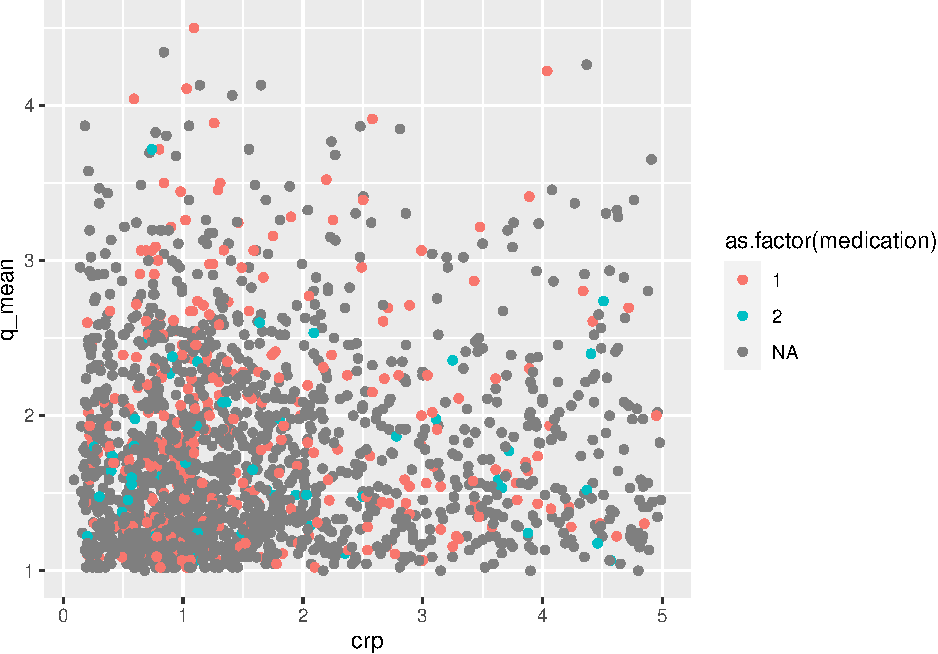
\includegraphics{Final_Groupof5_files/figure-latex/unnamed-chunk-9-1.pdf}

The descriptive statistics for our sample look as follows:

\begin{longtable}[]{@{}
  >{\raggedright\arraybackslash}p{(\columnwidth - 6\tabcolsep) * \real{0.0437}}
  >{\raggedright\arraybackslash}p{(\columnwidth - 6\tabcolsep) * \real{0.1913}}
  >{\raggedright\arraybackslash}p{(\columnwidth - 6\tabcolsep) * \real{0.3825}}
  >{\raggedright\arraybackslash}p{(\columnwidth - 6\tabcolsep) * \real{0.3825}}@{}}
\caption{Descriptive statistics.}\tabularnewline
\toprule()
\begin{minipage}[b]{\linewidth}\raggedright
\end{minipage} & \begin{minipage}[b]{\linewidth}\raggedright
\end{minipage} & \begin{minipage}[b]{\linewidth}\raggedright
China
\end{minipage} & \begin{minipage}[b]{\linewidth}\raggedright
Mexico
\end{minipage} \\
\midrule()
\endfirsthead
\toprule()
\begin{minipage}[b]{\linewidth}\raggedright
\end{minipage} & \begin{minipage}[b]{\linewidth}\raggedright
\end{minipage} & \begin{minipage}[b]{\linewidth}\raggedright
China
\end{minipage} & \begin{minipage}[b]{\linewidth}\raggedright
Mexico
\end{minipage} \\
\midrule()
\endhead
N & & 7196 & 1828 \\
Sex & & & \\
& male & 3466 (48.20 \%) & 39.50 (39.50 \%) \\
& female & 3723 (51.70 \%) & 60.40 (60.40 \%) \\
& unknown & 7 (0.10 \%) & 1 (0.10 \%) \\
Age & & 63 (SD = 9.30) & 67.70 (SD = 9) \\
Diabetes & & & \\
& diagnosed & 494 (6.90 \%) & 374 (20.50 \%) \\
& undiagnosed & 466 (6.50 \%) & 182 (10 \%) \\
\bottomrule()
\end{longtable}

\hypertarget{discussion}{%
\section{Discussion}\label{discussion}}

Enter text/code here.

\newpage

\hypertarget{references}{%
\section{References}\label{references}}




\hypertarget{refs}{}
\begin{CSLReferences}{1}{0}
\leavevmode\vadjust pre{\hypertarget{ref-example_ref}{}}%
Deshpande, A. D., Harris-Hayes, M., \& Schootman, M. (2008). Epidemiology of diabetes and diabetes-related complications. \emph{Physical Therapy}, \emph{88}(11), 1254--1264.

\end{CSLReferences}


\clearpage
\renewcommand{\listfigurename}{Figure captions}
\listoffigures
\clearpage
\renewcommand{\listtablename}{Table captions}
\listoftables

\end{document}
